\section{Introduction}

As part of the NSF-supported NDN ``Next Phase'' research from 2014-2016, 
the NDN project team has selected two network environments, {\bf Open mHealth} and {\bf
Enterprise Building Automation \& Management}, and one application
cluster, {\bf Mobile Multimedia}, to drive our research, verify the
architecture design, and ground evaluation of the next phase of our project.
The two environments represent critical areas in the design space for
next-generation Health IT and Cyberphysical Systems, respectively.  They
also extend work started in the previous NDN FIA project on participatory
sensing and instrumented environments to focus on specific application
ecosystems where we believe NDN can address fundamental challenges that
are unmet by IP.  Based on the successful initial results of previous
NDN research, we have identified Mobile  Multimedia as an application
area of cross-cutting relevance, motivated not only by the
network environments above but our team's desire to further develop
NDN by using it for our everyday communication.

This technical report provides background information on the {\bf Enterprise Building Automation and Management}
network environment including key application challenges faced using
IP and describes the design for a pilot application that the NDN team is 
building.  It serves as the primary design document for this application. 

\subsection{EBAMS Background}

%\begin{figure*}
%\begin{center}
\begin{wrapfigure}{r}{0.6\textwidth}
\vskip -12pt
%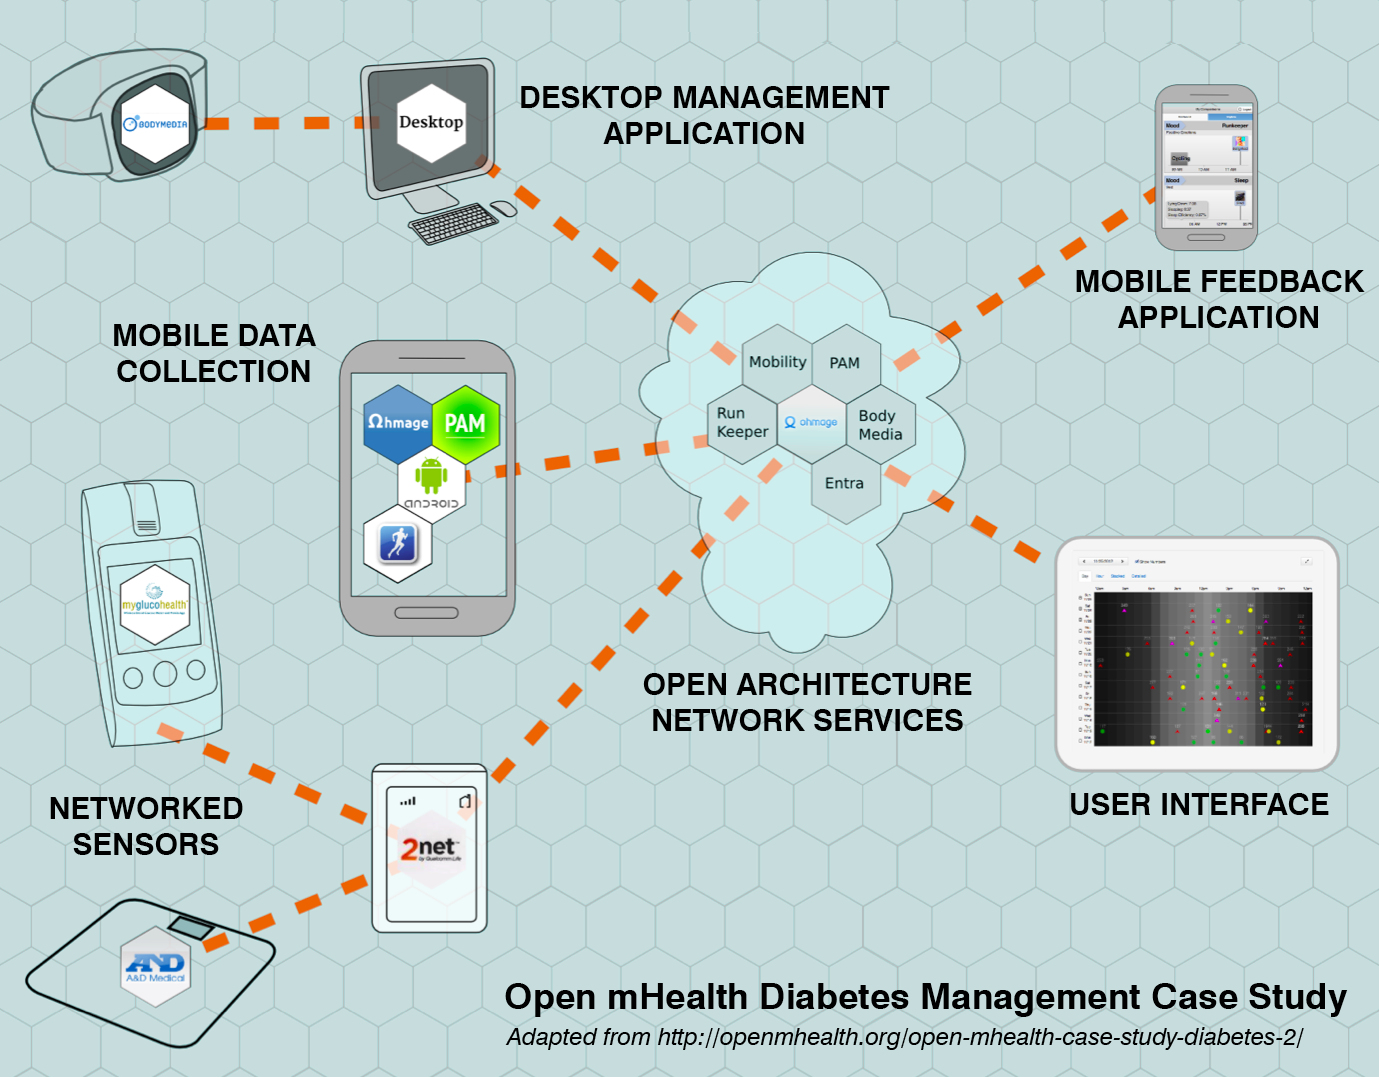
\epsfig{file=figures/OpenmHealth-figure.eps,width=.48\textwidth}
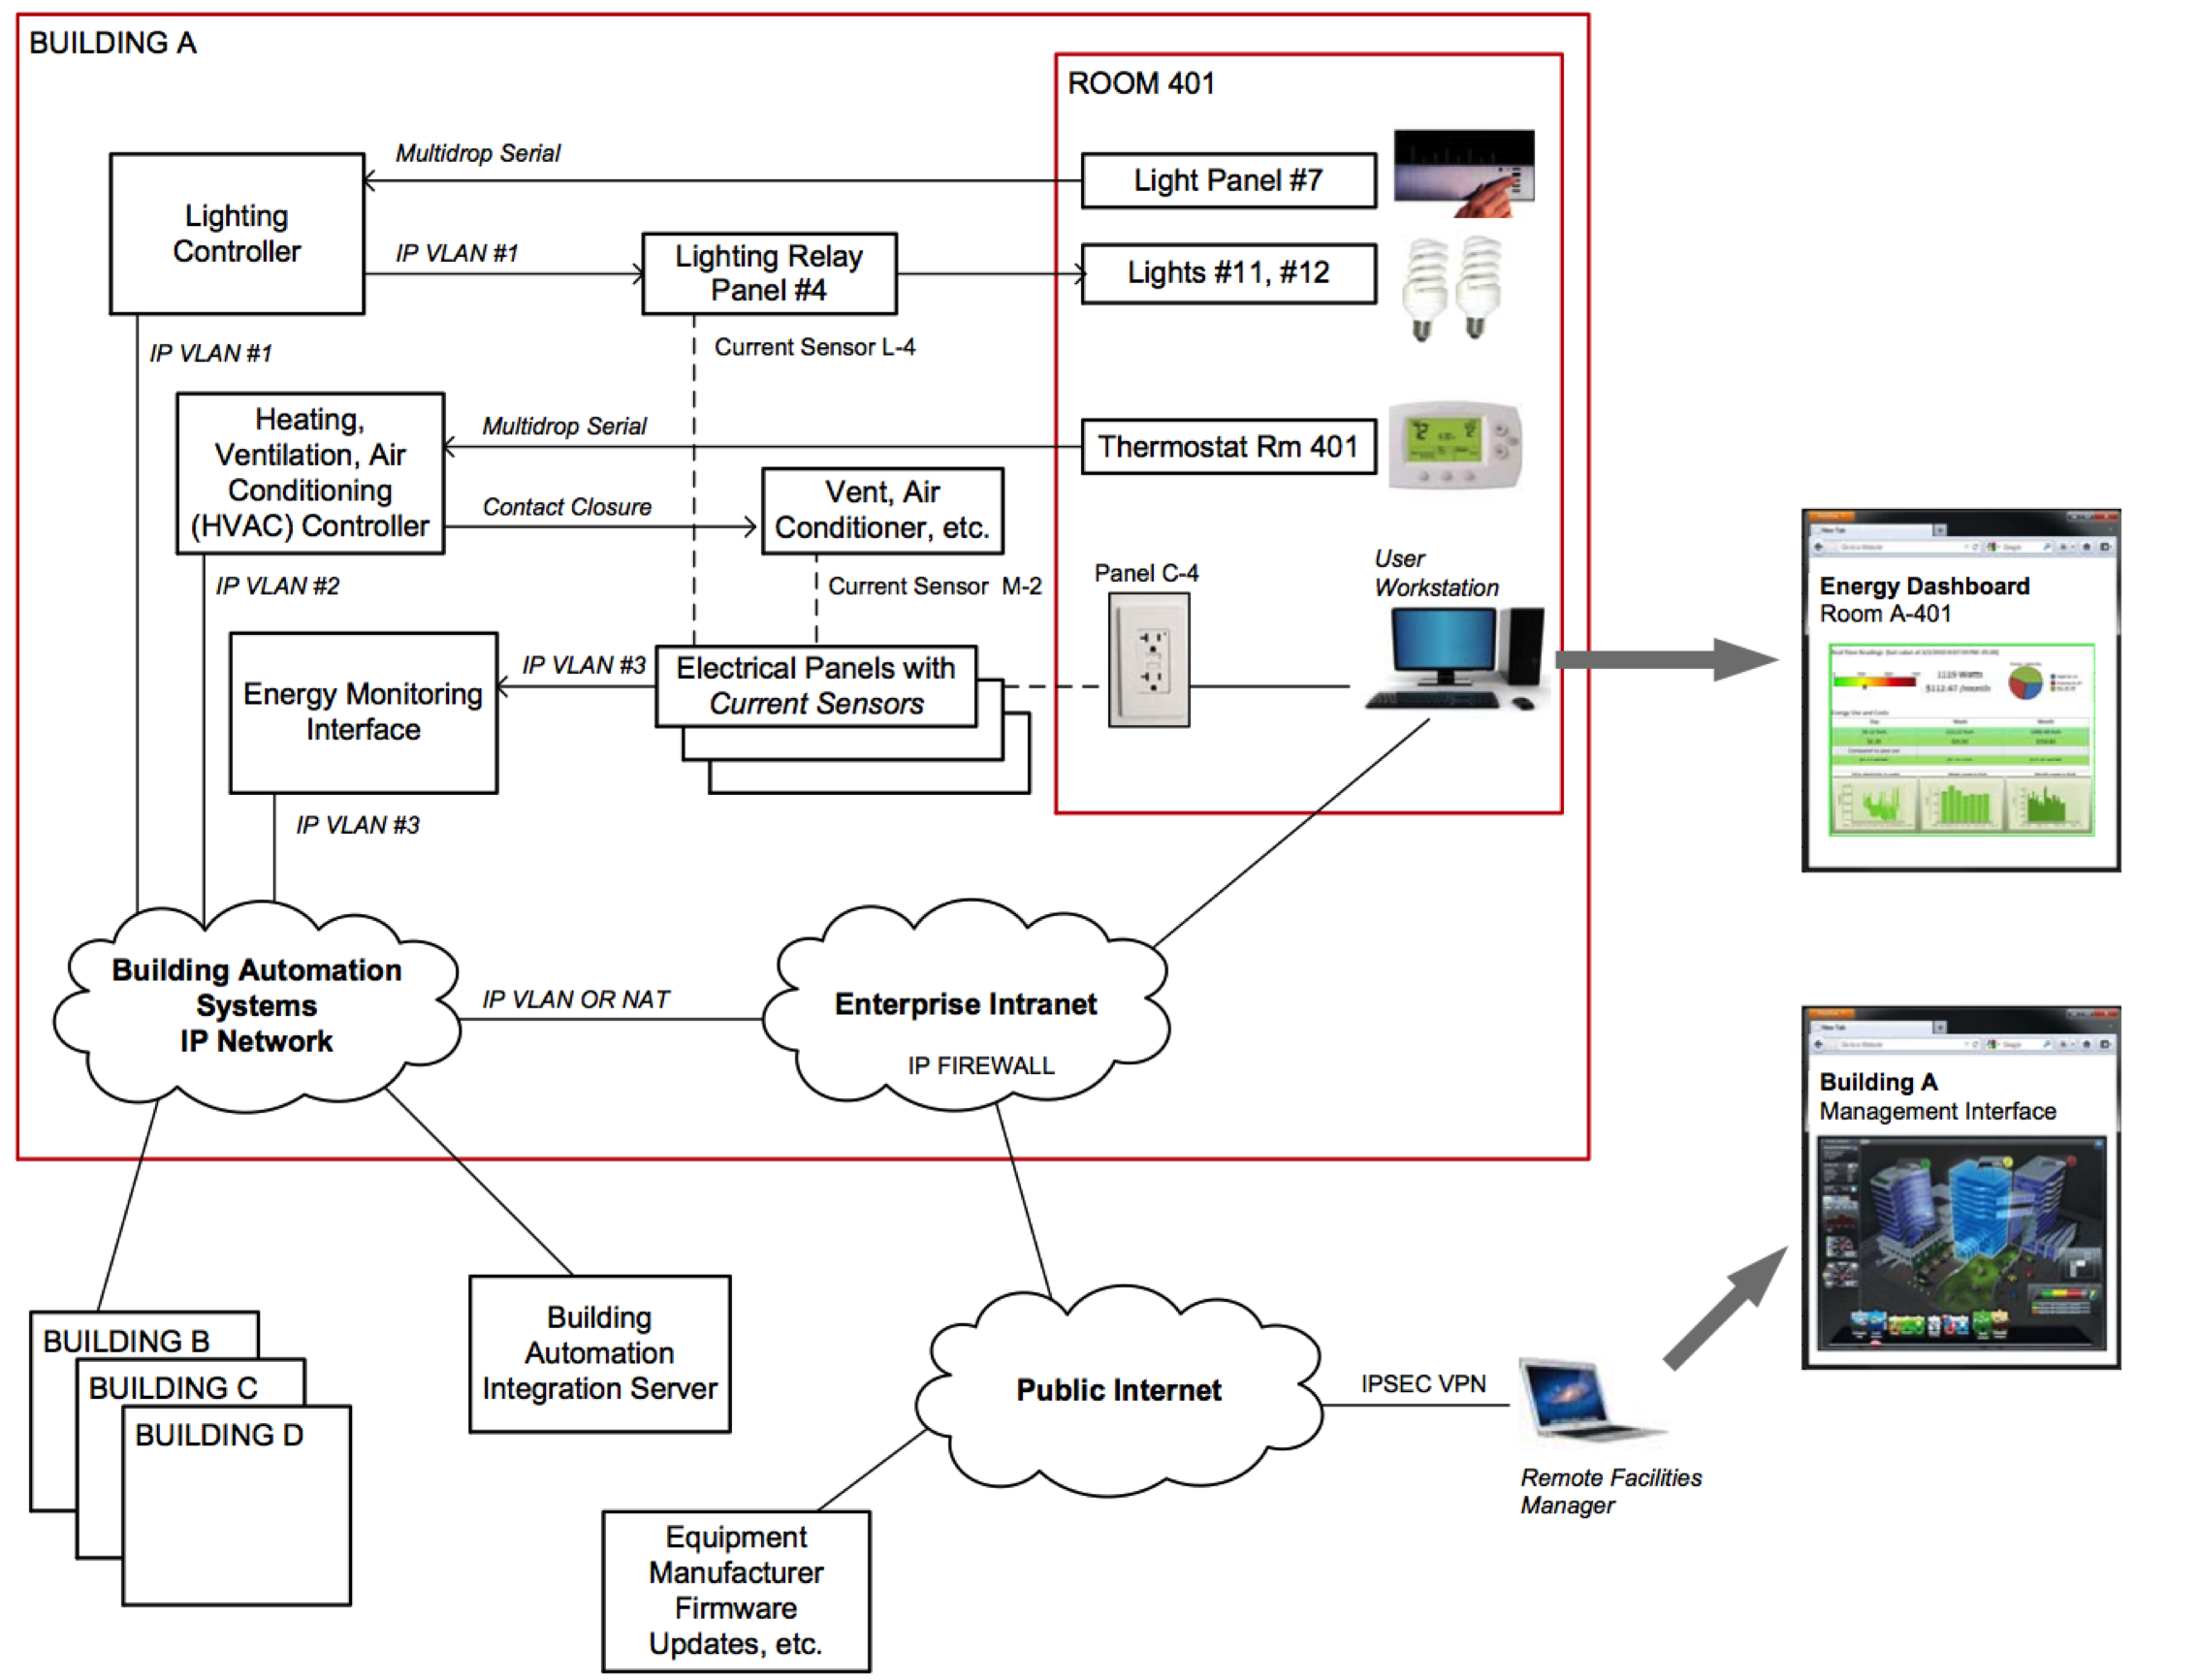
\includegraphics[width=.6\textwidth]{figures/BAS-Figure}
\vskip -5pt
\caption{{Example of building automation and management components, including sensors, controllers, and interfaces to both the public Internet and an enterprise intranet.  Securely integrating these heterogeneous components, while simplifying application development, is an important challenge posed by this network environment.}}
\label{fig:BAS}
\end{wrapfigure}
%\end{center}
%\end{figure*}

For our purposes, Enterprise Building Automation and Management covers the intersection of three critical sub-areas: \emph{industrial control systems} (ICS), including supervisory control and data acquisition (SCADA) and so-called smart grid~\cite{fang2011smart}, \emph{enterprise networking}, and the \emph{Internet of Things} (IOT) movement~\cite{atzori2010internet}. Enterprise BAS and BMS are environments that bring both critical infrastructure considerations of ICS with exciting visions for the everyday built environment of IoT.  In this domain, significant engineering challenges have emerged along with the promise offered by the convergence of networking in ICS with traditional IT, a sea change described by NIST in their ICS security review~\cite{NIST_ICS}.  

BAS and BMS are software/hardware systems that perform control, monitoring and management of heating, ventilation and air conditioning (HVAC), lighting, water, physical access and other building components. Their distributed, heterogeneous nature leads to a variety of challenges.  The IP protocol suite is increasingly used to network their components and as such is now a fundamental substrate of new buildings. However, IP networks suffer from limitations that impact innovation and trust in networked building systems, which we believe can be addressed with NDN.    
 
BAS/BMS pose complementary challenges to those of mHealth. They integrate hundreds to thousands of data collection and control points often implemented by special-purpose embedded devices and managed by a single enterprise.  Some devices are mobile and others are fixed; some devices are power-constrained and wireless while others are hard-wired and continuously communicating. Figure~\ref{fig:BAS} shows a few components of a typical system, including thermostats used for adjusting HVAC, lighting control and energy monitoring. 

Security is a fundamental and critical challenge~\cite{knapp2011industrial}. 
Like other ICS, BAS/BMS typically employ physical or logical isolation of the network as a primary security measure, which limits interoperability and integration.\footnote{In many cases, systems are left exposed to the Internet inadvertently. Only a few searches on \url{http://shodanhq.com/} make this abundantly clear.}   They also use a mixture of proprietary and open protocols, only a few of which offer intrinsic security. In many networks, there is no intrinsic security at lower layers, and only channel- and perimeter-based security above that, via SSL/TLS, VPNs, and routing configuration. Given the importance of integrating subsystems for applications such as energy management, fault detection, and synchronization,  network segregation and closed protocols are not a viable long-term approach. Figure~\ref{fig:BAS} shows an environment that supports access to control and monitoring from intranet web sites, but makes ``air gaps'' impossible and logical network separation hard to engineer and maintain for normal enterprises. 
%@@jeff: don't you mean makes air gaps possible above? 

For application developers, there is a fundamental mismatch in BAS/BMS between how network applications are authored (typically data-centric) vs.~fieldbus and IP network abstractions (host- and device-centric).  
	%@@jeff: i dont know what fieldbus is.  will most reviewers?
Addressing is spread across many layers, most of which are not routable. There is a great heterogeneity in protocols, especially at the fieldbus level.  Typically, application developers and platform manufacturers implement abstraction layers in middleware \cite{Sauter2010}, often complex, proprietary, and challenging to configure.

%not address the network configuration
%Indeed, in many practical scenarios, BAS platform manufacturers develop middleware that abstracts away the addressing and protocol details. 
%, as described in the following paragraph.
%, as is IP subnetting and routing, which reflect device organization and interconnectivity. 
%are typically invisible or inaccessible to applications.

In addition to the protocols themselves, significant application logic is bound up in network configuration not accessible to developers or users: 1) VLANs, IP subnetting, and routing configurations enforce boundaries between systems;
2) firewall configurations describe brittle rules for system access, which can be difficult to change; 3) keys and certificates for SSL connections and VPNs may identify connections; 4) VPN configuration and enterprise authentication hold remote network access permissions. None of these are typically visible or accessible to application software in traditional systems. In fact, they represent important system control logic that is often replicated ad-hoc in application configurations. A simple example is how an application must be configured to know that 192.168.2.1/24 is lighting and 192.168.3.1/24 is HVAC, which is site-specific and meaningless to an application.  Such configurations also bring brittleness to changing topologies and devices.

Our selection of digitally-controlled cyberphysical systems  as a
network environment is inspired by the practical goal of enabling more 
efficient operation of buildings, improved comfort and control for occupants, 
and new opportunities for understanding the interactions between elements 
of our built environment. 

\subsection{Relationship to NDN-IoT}

The EBAMS research has much in common with the ``Internet of Things'' (IoT) vision and related NDN research.  For now, we consider IoT applications separately (and not in this document), motivated from consumer experience and smart home deployments.  That research focuses on a bottom-up approach to networking devices using NDN, including issues such as NDN support on resource-constrained devices, bootstrapping and name assignment.  The EBAMS network environment focuses on enterprise-scale networking of industrial control and monitoring technologies. 

Figure~\ref{fig:apogee-levels} shows the ``levels'' of an industry-standard Siemens Apogee system.  Our NP research focuses on the ``management'' and ``automation'' levels, while the IoT work has more in common with the ``field'' level .

\begin{figure*}
\begin{center}
\vskip -12pt
%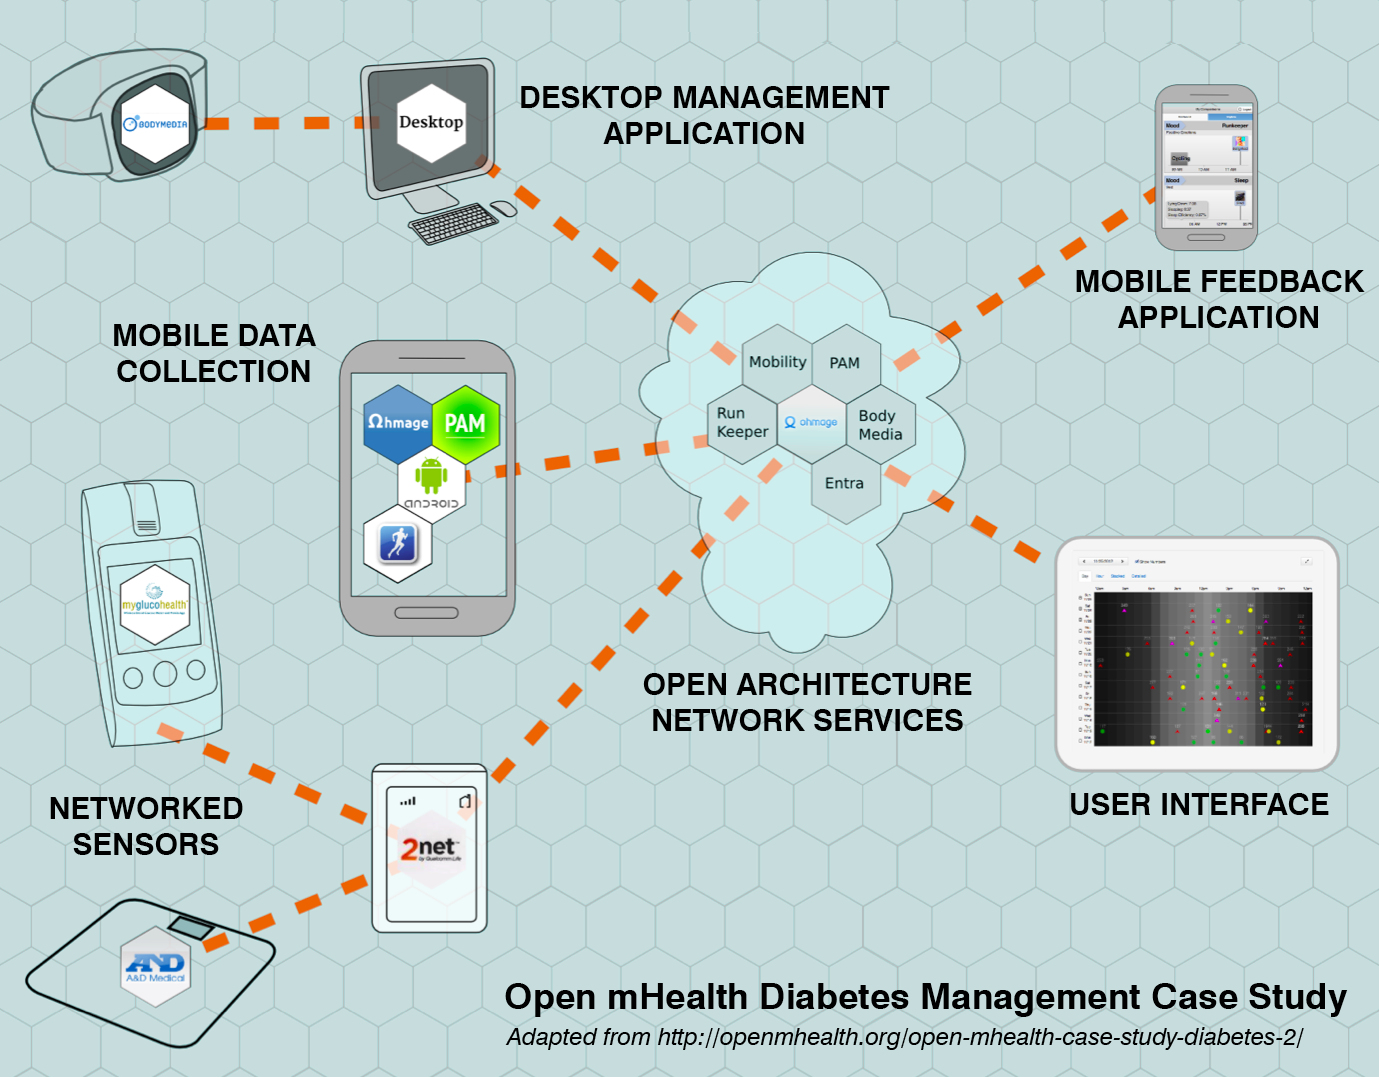
\epsfig{file=figures/OpenmHealth-figure.eps,width=.48\textwidth}
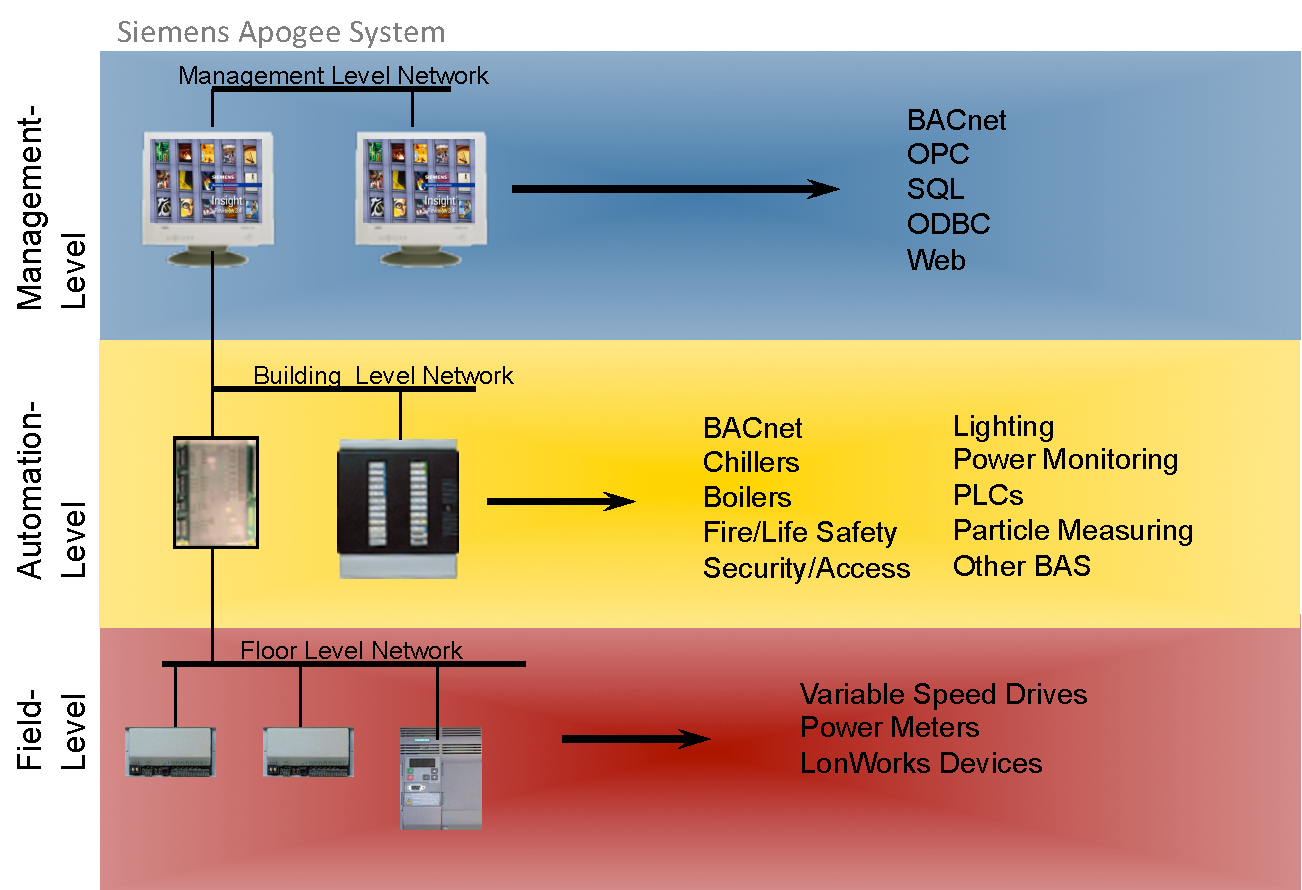
\includegraphics[width=.6\textwidth]{figures/siemens-apogee-levels}
\vskip -5pt
\caption{{Levels in a Siemens Apogee system. The EBAMS network environment focuses on the ``management'' and ``automation'' levels.}}
\label{fig:apogee-levels}
\end{center}
\end{figure*}

\subsection{Challenges of IP}

\begin{itemize}
\item \textbf{Addressing spread across many layers} (e.g., VLAN, host IP, port, device number, etc.) that over-emphasizes gateways over actual sensors/actuators.  
\item Legacy protocols \textbf{rely on logical / physical isolation} of control and monitoring networks from IT systems. Use of IP protocol provides many new integration possibilities but new security risks;  \textbf{traditional perimeter and channel-based security insufficient}. 
\item Many devices don’t have user interfaces. \textbf{Discovery and bootstrapping} still relies on DHCP, TFTP, etc. or manual configuration. 
\item Middleware has been proprietary and often heavyweight.  To get data-centric communication, often building on SOAP/HTTP, etc. 
\item COAP also proposes a request-response model but still the \textbf{channel-based security} of DTLS as the primary approach, with IPSec as an alternative.    Multicast support is limited across all of these options. 
\end{itemize}

\subsection{Benefits of NDN}

\begin{itemize}
\item Massive \textbf{addressing simplification}, with a potential for huge impact when scaled to the enterprise. Simpler network infrastructure needed to deploy complex monitoring and automation. 
\item New ways of working with edge resources that \textbf{de-emphasize gateway addressing} while preserving support for topological heterogeneity. 
\item Lighter-weight, \textbf{data-centric security} options easier to develop, with data verification intrinsically part of the architecture. 
\item \textbf{Caching and storage integration} may provide significant advantages in distributed storage at all levels of the architecture, increasing \item data availability without power increase. 
\item Intrinsic multicast; \textbf{many-to-many communication easier to deploy}. 
\end{itemize}

\subsection{Collaboration}

UCLA Facilities Management has agreed to act as domain experts and help define the practical requirements of this network environment.  UCLA's currently deployed building management system has approximately 150,000 points of monitoring across the campus, potentially growing to over 400,000 points in the next five years.  It is the largest installation on the West Coast for Siemens building systems after Microsoft.  UCLA's IT, DDC (direct digital control), and engineering staff will interact with the NDN team to enumerate their requirements, challenges, and limitations.  As part of the previous EAGER award, UCLA FM has already helped us install a dedicated Siemens electrical demand monitoring system for a laboratory space for research.  We expect they will also help us install a dedicated server that will provide near real-time access to ~20,000 points worth of data from campus' operational systems, probably about 10 buildings worth of data.  We plan to use this server as a gateway to our own NDN testbed. 

Pilot application collaboration:
\begin{itemize}
\item UCLA REMAP
\item UCLA IRL
\item U. Michigan
\item U. Arizona
\item U. Memphis
\item WUSTL
\end{itemize}

\subsection{Proposed Milestones 2014-2016}

\begin{itemize}
\item Review limitations in current IP-based architecture, for Facilities Management needs. (Y1)
\item Design NDN namespace, repository, trust and communication model for use cases, such as energy management, new building commissioning, feedback control. (Y1; updated in Y2)
\item Implement low-level NDN applications, such as energy management data gathering. (Y1)
\item Preliminary embedded platform support. (Y2)
\item Integrate “live” UCLA building data into the NDN testbed, mirroring data from 10-20 UCLA buildings. (Y2)
\item Implement high-level NDN application for enterprise building monitoring, based on the above data, applying distributed 3D visualization work done in the first FIA project. (Y2)
\end{itemize}


